\documentclass[nofootinbib,amssymb,amsmath]{revtex4}
\usepackage{mathtools}
\usepackage{amsthm}
\usepackage{algorithm}
\usepackage{algpseudocode}
\usepackage{lmodern}
\usepackage{graphicx}
\usepackage{color}
\usepackage{bm}

%Put an averaged random variable between brackets
\newcommand{\ave}[1]{\left\langle #1 \right\rangle}

\newcommand{\vzero}{{\bf 0}}
\newcommand{\vI}{{\bf I}}
\newcommand{\vb}{{\bf b}}
\newcommand{\vd}{{\bf d}}
\newcommand{\vf}{{\bf f}}
\newcommand{\vc}{{\bf c}}
\newcommand{\vv}{{\bf v}}
\newcommand{\vz}{{\bf z}}
\newcommand{\vn}{{\bf n}}
\newcommand{\vm}{{\bf m}}
\newcommand{\vG}{{\bf G}}
\newcommand{\vQ}{{\bf Q}}
\newcommand{\vM}{{\bf M}}
\newcommand{\vW}{{\bf W}}
\newcommand{\vX}{{\bf X}}
\newcommand{\vPsi}{{\bf \Psi}}
\newcommand{\vSigma}{{\bf \Sigma}}
\newcommand{\vlambda}{{\bf \lambda}}
\newcommand{\vpi}{{\bf \pi}}
\newcommand{\valpha}{{\bm{\alpha}}}
\newcommand{\vbeta}{{\bm{\beta}}}
\newcommand{\vomega}{{\bm{\omega}}}
\newcommand{\vLambda}{{\bf \Lambda}}
\newcommand{\vA}{{\bf A}}

\newcommand{\code}[1]{\texttt{#1}}
\newcommand*{\Comb}[2]{{}^{#1}C_{#2}}

\newtheorem{lemma}{Lemma}
\newtheorem{corollary}{Corollary}

\def\SL#1{{\color [rgb]{0,0,0.8} [SL: #1]}}
\def\DB#1{{\color [rgb]{0,0.8,0} [DB: #1]}}

\newcommand{\HOM}{$\mathsf{Hom}$}
\newcommand{\HET}{$\mathsf{Het}$}
\newcommand{\REF}{$\mathsf{Ref}$}
\newcommand{\epss}{\varepsilon}

\begin{document}

\title{Mathematical Notes on Mutect}
\author{David Benjamin}
\email{davidben@broadinstitute.org}
\affiliation{Broad Institute, 75 Ames Street, Cambridge, MA 02142}
\author{Takuto Sato}
\email{tsato@broadinstitute.org}
\affiliation{Broad Institute, 75 Ames Street, Cambridge, MA 02142}

\date{\today}

\maketitle

\section{Somatic Likelihoods Model}\label{introduction}

We have a set of potential somatic alleles and read-allele likelihoods $\ell_{ra} \equiv P({\rm read~}r|{\rm allele~}a)$.  We don't know which alleles are real somatic alleles and so we must compute, for each subset $\mathbb{A}$ of alleles, the likelihood that the reads come from $\mathbb{A}$.  A simple model for this likelihood is as follows: each read $r$ is associated with a latent indicator vector $\vz_r$ with one-hot encoding $z_{ra} = 1$ iff read $r$ came from allele $a \in \mathbb{A}$.  The conditional probability of the reads $\mathbb{R}$ given their allele assignments is
\begin{equation}
P( \mathbb{R} | \vz, \mathbb{A}) = \prod_{r \in \mathbb{R}} \prod_a \ell_{ra}^{z_{ra}}.
\end{equation}
The alleles are not equally likely because there is a latent vector $\vf$ of allele fractions -- $f_a$ is the allele fraction of allele $a$.  Since the components of $\vf$ sum to one it is a categorical distribution and can be given a Dirichlet prior,
\begin{equation}
P(\vf) = {\rm Dir}(\vf | \valpha).
\end{equation}
Then $f_a$ is the prior probability that a read comes from allele $a$ and thus the conditional probability of the indicators $\vz$ given the allele fractions $\vf$ is
\begin{equation}
P(\vz | \vf) = \prod_r \prod_a f_a^{z_{ra}}.
\end{equation}
The full-model likelihood is therefore
\begin{equation}
\mathbb{L}(\mathbb{A}) = P(\mathbb{R}, \vz, \vf | \mathbb{A}) = {\rm Dir}(\vf | \valpha) \prod_a  \prod_r \left( f_a \ell_{ra}\right)^{z_{ra}}.
\label{full_likelihood}
\end{equation}
And the marginalized likelihood of $\mathbb{A}$, that is, the model evidence for allele subset $\mathbb{A}$, is
\begin{equation}
P(\mathbb{R} | \mathbb{A}) = \sum_\vz \int d \vf \, {\rm Dir}(\vf | \valpha) \prod_a  \prod_r \left( f_a \ell_{ra}\right)^{z_{ra}},
\label{evidence}
\end{equation}
where the integral is over the probability simplex $\sum_a f_a = 1$.

The integral over $\vf$ is the normalization constant of a Dirichlet distribution and as such we can simply look up its formula.  However, the sum over all values of $\vz$ for all reads has exponentially many terms.  We will get around this difficulty by handling $\vz$ with a mean-field approximation in which we factorize the likelihood as $\mathbb{L} \approx q(\vz) q(\vf)$.  This approximation is exact in two limits: first, if there are many reads, each allele is associated with many reads and therefore the Law of Large Numbers causes $\vf$ and $\vz$ to become uncorrelated.  Second, if the allele assignments of reads are obvious $\vz_r$ is effectively not a random variable at all (there is no uncertainty as to which of component is non-zero) and also becomes uncorrelated with $\vf$.

In the variational Bayesian mean-field formalism the value of $\vf$ that $\vz$ ``sees'' is the expectation of $\log \mathbb{L}$ with respect to $q(\vf)$ and vice versa.  That is,
\begin{equation}
q(\vf) \propto {\rm Dir}(\vf | \valpha) \prod_a  \prod_r f_a^{\bar{z}_{ra}} \propto {\rm Dir}(\vf | \valpha + \sum_r \bar{\vz}_r),
\label{qf}
\end{equation}
where $\bar{z}_{ra} \equiv E_q \left[ z_{ra} \right]$, and
\begin{equation}
q(\vz_r) = \prod_a \left( \tilde{f}_a \ell_{ra}\right)^{z_{ra}}, \tilde{f}_a = \exp E[\ln f_a]
\end{equation}
Because $q(\vz)$ is categorical and $q(\vf)$ is Dirichlet\footnote{Note that we didn't \textit{impose} this in any way.  It simply falls out of the mean field equations.} the necessary mean fields are easily obtained and we have
\begin{equation}
\bar{z}_{ra} = \frac{\tilde{f}_a \ell_{ra}}{\sum_{a^\prime} \tilde{f}_{a^\prime} \ell_{ra^\prime}}
\label{z_mean_field}
\end{equation}
and
\begin{equation}
\ln \tilde{f}_a = \psi(\alpha_a + \sum_r \bar{z}_{ra}) - \psi(\sum_{a^\prime} \alpha_{a^\prime} + N)
\label{f_mean_field}
\end{equation}
where $\psi$ is the digamma function and $N$ is the number of reads.  To obtain $q(\vz)$ and $q(\vf)$ we iterate Equations \ref{z_mean_field} and \ref{f_mean_field} until convergence.  A very reasonable initialization is to set $\bar{z}_{ra} = 1$ if $a$ is the most likely allele for read $r$, 0 otherwise.  Having obtained the mean field of $\vz$, we would like to plug it into Eq \ref{evidence}.  We can't do this directly, of course, because Eq \ref{evidence} says nothing about our mean field factorization.  Rather, we need the variational approximation (Bishop's Eq 10.3) to the model evidence, which is
\begin{align}
\ln P(\mathbb{R} | \mathbb{A}) \approx& \sum_{\vz} \int d \vf q(\vz) q(\vf) \left[ \ln P(\mathbb{R}, \vz, \vf | \mathbb{A}) - \ln q(\vz) - \ln q(\vf) \right] \\
=& E_q \left[ \ln P(\mathbb{R}, \vz, \vf | \mathbb{A}) \right] - E_q \left[ \ln q(\vz) \right] - E_q \left[ \ln q(\vf) \right]. \label{lagrangian}
\end{align}
Before we proceed, let's introduce some notation.  First, from Eq \ref{qf} the posterior $q(\vf)$ is
\begin{equation}
q(\vf) = {\rm Dir}(\vf | \vbeta), \quad \vbeta = \valpha + \sum_r \bar{\vz}_r.
\end{equation}
Second, let's define the log normalization constant of a Dirichlet distribution as $g$ so that
\begin{equation}
\ln {\rm Dir}(\vf | \vomega) = g(\vomega) + \sum_a (\omega_a - 1) \ln f_a, \quad g(\vomega) = \ln \Gamma(\sum_a \omega_a) - \sum_a \ln \Gamma(\omega_a).
\end{equation}
Finally, define the Dirichlet mean log (aka ``that digamma stuff") as $h$:
\begin{equation}
E_{\rm Dir(\vf | \vomega)} \left[ \ln f_a \right] = \psi(\omega_a) - \psi(\sum_{a^\prime} \omega_{a^\prime}) \equiv h_a(\vomega).
\end{equation}

The log of Eq \ref{full_likelihood} is
\begin{equation}
\ln P(\mathbb{R}, \vz, \vf | \mathbb{A}) = g(\valpha) + \sum_a (\alpha_a - 1) \ln f_a + \sum_{ra} z_{ra} (\ln f_a + \ln \ell_{ra}).
\end{equation}
and thus the first term in Eq \ref{lagrangian} is
\begin{align}
E_q \left[ \ln P(\mathbb{R}, \vz, \vf | \mathbb{A}) \right] =& g(\valpha) + \sum_a (\alpha_a - 1) h_a(\vbeta) + \sum_{ra}\bar{z}_{ra} \left( h_a(\vbeta) + \ln \ell_{ra} \right) \\
=& g(\valpha) + \sum_a (\beta_a - 1) h_a(\vbeta) + \sum_{ra}\bar{z}_{ra} \ln \ell_{ra}, \label{first_term}
\end{align}
where we used the relationship $\vbeta = \valpha + \sum_r \bar{\vz}_r$.

The second term in Eq \ref{lagrangian} is
\begin{align}
- E_q \left[ \ln q(\vz) \right] = - \sum_{ra} \bar{z}_{ra} \ln \bar{z}_{ra} \label{second_term}.
\end{align}

The third term in Eq \ref{lagrangian} is
\begin{align}
- E_q \left[ \ln q(\vf) \right] = -g(\vbeta) - \sum_a (\beta_a - 1) E_q [\ln f_a] = -g(\vbeta) - \sum_a (\beta_a - 1) h_a(\vbeta) \label{third_term}.
\end{align}

Adding Eqs \ref{first_term}, \ref{second_term}, and \ref{third_term} and noting the cancellation between parts of Eqs \ref{first_term} and \ref{third_term} we obtain
\begin{equation}
\ln P(\mathbb{R} | \mathbb{A}) \approx g(\valpha) - g(\vbeta) +  \sum_{ra} \bar{z}_{ra} \left( \ln \ell_{ra} - \ln \bar{z}_{ra} \right).
\end{equation}

We now have the model evidence for allele subset $\mathbb{A}$.  This lets us choose which alleles are true somatic variants.  It also lets us make calls on somatic loss of heterozygosity events.  Furthermore, instead of reporting max-likelihood allele fractions as before, we may emit the parameters of the Dirichlet posterior $q(\vf)$, which encode both the maximum likelihood allele fractions and their uncertainty.

\section{Strand Artifact Model}

\begin{figure}
\centering
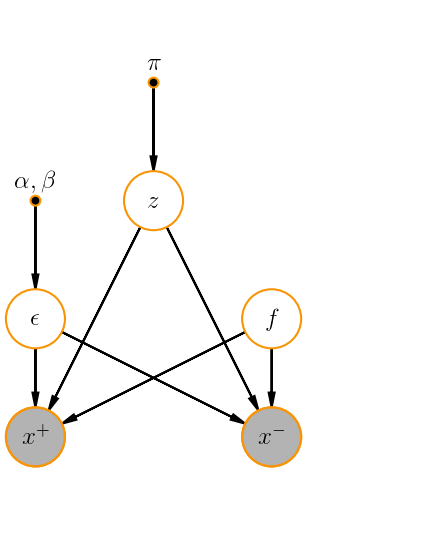
\includegraphics[width=0.3\textwidth]{strand_artifact_pgm.png}
\caption{\label{fig:strand artifact}The probabilistic graphical model for the strand artifact model}
\end{figure}

The strand artifact filter detects sequencing artifacts in which the evidence for the alt allele consists entirely of forward strand reads alone or reverse strand reads alone. We must detect this while taking into account the fact that at some loci, such as near the end of an exome target, \emph{all} reads are biased towards one direction, and therefore a bias towards a particular strand among alt reads is no cause for alarm.

Let $z \in \{ z_+, z_-, z_o \}$ be a latent random variable with 1-hot encoding that represents the artifact state of a suspected variant. $z_+ = 1$ when the candidate variant is a forward strand artifact, $z_- = 1$ when it's a reverse artifact, and $z_o = 1$ when there's no artifact. At each locus, the conditional distribution over the number of forward alt reads $x^+$ is a binomial random variable

\begin{equation}
P(x^+ | f, \epsilon, z) = \text{Bin} (x^+ | n^+, f + \epsilon(1-f))^{z_+} \text{Bin} (x^+ | n^+, f)^{1 - z_+}
\end{equation}

where $n^+$ is the number of \emph{total} forward reads, $f$ is the allele fraction, and $\epsilon$ is the artifactual error rate, which is the probability that we mistakenly read a ref allele as alt due to strand artifact. We put a flat prior on $f$ and a beta prior on $\epsilon$. The conditional distribution of $x^-$ is defined analogously.

In order to decide whether to filter a variant, we compute the posterior probabilities of $z$ given the observed alt read counts $X = \{ x^+, x^- \}$.  We obtain the likelihood $P(X | z)$ by marginalizing the latent variables $f$ and $\epsilon$ out of the joint distribution $P(X, f, \epsilon | z)$, and we do this for each of the three possible values of $z$ separately. First consider the case $z_+ = 1$, which we denote by the shorthand $z_+$ below.

\begin{align}
P(X | z_+ )  &= \iint  P(X, f, \epsilon | z_+) \,df\,d\epsilon \nonumber \\
		  &= \iint  P(f) P(\epsilon) P(x^+ | z_+, f, \epsilon) P(x^- | z_+, f, \epsilon) \,df\,d\epsilon \nonumber \\
		  &= \iint \mathrm{Beta}(\epsilon|\alpha, \beta) \mathrm{Bin}(x^+ | n^+, f + \epsilon(1-f)) \mathrm{Bin}(x^- | n^-, f) \,df\,d\epsilon
\end{align}

where $\alpha$ and $\beta$ are fixed hyperparameters to the beta prior on $\epsilon$. By Bayes Rule the posterior probability of strand bias for forward reads is therefore

\begin{align}
P(z_+ | X) & \propto P(z_+) P(X | z_+) = \pi_+ P(X | z_+) 
\end{align}

where $\pi_+ = P(z_+)$ is a fixed prior probability of strand artifact. The posterior probability of reverse strand artifact $P(z_- | X)$ may be derived analogously. 

The derivation of $P(z_o|X)$ is similar except that the integral becomes much simpler because $P(X|z_o)$ does not depend on the artifactual error rate $\epsilon$.

\begin{align}
P(X | z_o)  &= \iint P(\epsilon) P(x^+ | z_o, f, \epsilon) P(x^- | z_o, f, \epsilon) \,df\,d\epsilon \nonumber \\
	 	 &= \int  P(x^+ | z_o, f) P(x^- | z_o, f) \,df \int  P(\epsilon) d\epsilon \nonumber \\
		 &= \int  \mathrm{Bin}(x^+ | n^+, f) \mathrm{Bin}(x^- | n^-, f) \,df
\end{align}

And the posterior probability is

\begin{equation}
P(z_o | X) \propto P(z_o) P(X | z_o) =  \pi_o P(X | z_o) 
\end{equation}

where $\pi_o = P(z_o = 1)$ is the fixed prior probability of no artifact. We normalize the posteriors and filter the variant if the posterior probability of $z_+ = 1$ or $z_- = 1$ exceeds the threshold.

\section{Germline Filter}\label{germline-filter}
Suppose we have detected an allele such that its (somatic) likelihood in the tumor is $\ell_t$ and its (diploid) likelihood in the normal is $\ell_n$\footnote{This is the total likelihood for het and hom alt in the normal.}.  By convention, both of these are relative to a likelihood of $1$ for the allele \textit{not} to be found.  If we have no matched normal, $\ell_n = 1$.  Suppose we also have the population allele frequency $f$ of this allele.  Then the prior probabilities for the normal to be heterozygous and homozygous alt for the allele are $2f(1-f)$ and $f^2$ and the prior probability for the normal genotype not to contain the allele is $(1-f)^2$.  Finally, suppose that the prior for this allele to arise as a somatic variant is $\pi$.

We can determine the posterior probability that the variant exists in the normal genotype by calculating the unnormalized probabilities of four possibilities:
\begin{enumerate}
\item The variant exists in the tumor and the normal as a germline het.  This has unnormalized probability $2f(1-f) \ell_n \ell_t (1 - \pi)$.
\item The variant exists in the tumor and the normal as a germline hom alt.  This has unnormalized probability $f^2 \ell_n \ell_t (1 - \pi)$.
\item The variant exists in the tumor but not the normal.  This has unnormalized probability $(1-f)^2 \ell_t \pi$.
\end{enumerate}

We exclude possibilities in which the variant does not exist in the tumor sample because we really want the conditional probability that the variant is germline given that it would otherwise be called.

Normalizing, we obtain the following posterior probability that an allele is a germline variant:
\begin{equation}
P({\rm germline}) = \frac{(1) + (2)}{(1) + (2) + (3)} = \frac{\left(2f(1-f) + f^2 \right) \ell_n \ell_t (1 - \pi)}{\left(2f(1-f) + f^2 \right) \ell_n \ell_t  (1 - \pi) + \ell_t (1-f)^2  \pi}.
\end{equation}

The above equation, in which the factors of $\ell_t$ could cancel if we wished, is not quite right.  The tumor likelihood $\ell_t$ is the probability of the tumor data given that the allele exists in the tumor \textit{as a somatic variant}.  If the allele is in the tumor as a germline het we must modify $\ell_t$ to account for the fact that the allele fraction is determined by the ploidy -- it must be either $f_g$ or $1- f_g$with equal probability, where $f_g$ is the minor allele fraction of germline hets.  It would be awkward to recalculate the tumor likelihood with the allele frequency constrained to these two values\footnote{The model could easily accommodate this change, but the likelihoods are long gone from memory once the germline computation occurs.}, but we can estimate a correction factor as follows:  assuming that the posterior on the allele fraction in the somatic likelihoods model is fairly tight, the likelihood of $a$ alt reads out of $n$ total reads is $\binom na (1-f_t)^{n-a}f^a$, where $f_t$ is the tumor alt allele fraction.  That is, our sophisticated model that marginalizes over $f_t$ reduces to something more naive.  If the variant is a germline event, the likelihood becomes $\frac{1}{2} \binom na  \left[(1-f_g)^{n-a}f_g^a + f_g^{n-a}(1-f_g)^a \right]$.  Thus, in case (1) we have $\ell_t \rightarrow \chi \ell_t$, where
\begin{equation}
\chi = \frac{1}{2} \frac{(1-f_g)^{n-a}f_g^a + f_g^{n-a}(1-f_g)^a}{(1-f_t)^{n-a}f_t^a}.
\end{equation}
For germline hom alts, both the tumor and normal allele fractions will be similarly large, so to decent approximation we don't have to modify $\ell_t$.  Of course, this only applies if the allele fraction is large.  Rather than try to model the count of ref reads within a germline hom alt site, we simply set a threshold of allele fraction 0.9, so that in case (2) $\ell_t \rightarrow {\rm I}[f_t > 0.9] \ell_t$.
and the corrected germline probability is
\begin{equation}
P({\rm germline}) = \frac{(1) + (2)}{(1) + (2) + (3)} = \frac{\left( 2f(1-f) \chi + {\rm I}[f_t > 0.9] f^2 \right) \ell_n (1 - \pi)}{\left( 2f(1-f) \chi + {\rm I}[f_t > 0.9] f^2 \right) \ell_n  (1 - \pi) + (1-f)^2  \pi}.
\end{equation}
To filter, we set a threshold on this posterior probability.

So far we have assumed that the population allele frequency $f$ is known, which is the case if it is found in our germline resource, such as gnomAD.  If $f$ is not known we must make a reasonable guess as follows.  Suppose the prior distribution on $f$ is ${\rm Beta}(\alpha, \beta)$.  The mean $\alpha/(\alpha +\beta)$ of this prior is the average human heterozygosity $\theta \approx 10^{-3}$, so we have $\beta \approx \alpha / \theta$.  We need one more constraint to determine $\alpha$ and $\beta$, and since we are concerned with imputing $f$ when $f$ is small we use a condition based on rare variants.  Specifically, the number of variant alleles $n$ at some site in a germline resource with $N/2$ samples, hence $N$ chromosomes, is given by $f \sim {\rm Beta}(\alpha, \beta), n \sim {\rm Binom}(N,f)$.  That is, $n \sim {\rm BetaBinom}(\alpha, \beta, N)$.  The probability of a site being non-variant in every sample is then $P(n = 0) = {\rm BetaBinom}(0 | \alpha, \beta, N)$, which we equate to the empirical proportion of non-variant sites in our resource, about $7/8$ for exonic sites in gnomAD.  Solving, we obtain approximately $\alpha = 0.01, \beta = 10$ for gnomAD.  Now, given that some allele found by Mutect is not in the resource, the posterior on $f$ is ${\rm Beta}(\alpha, \beta + N)$, the mean of which is, since $\beta << N$, about $\alpha / N$.  By default, Mutect uses this value.

\section{Contamination Filter}\label{contamination-filter}
Suppose our tumor bam has contamination fraction $\alpha$ and that at some site we have $a$ alt reads out of $d$ total reads.  Suppose further that the alt allele has population allele frequency $f$.  We will compute a simple estimate of the posterior probability that these alt reads came from a contaminating sample and not from a true somatic variant.  Let $\pi$ be the prior probability of somatic variation as above.  Our crude model for the alt count distribution of somatic variation is a uniform distribution.  That is, we assume that any value of $a$ from $0$ to $d$ is equally likely.  Then the likelihood of the data given a true somatic variant is
\begin{equation}
P(a | {\rm somatic})  = \frac{1}{d + 1}.
\end{equation}

We consider two models of contamination.  If there are multiple contaminants we approximate each contaminant read as independent.  Then the probability of any given read being an alt contaminant read is $\alpha f$, so we have
\begin{equation}
P(a | {\rm many~contaminant}) = {\rm Binom}(a | d, \alpha f).
\end{equation}
If there is a single contaminating sample it is heterozygous with probability $2f(1-f)$ and homozygous for the alt with probability $f^2$, in which cases fractions $\alpha/2$ and $\alpha$ of all reads to be alt contaminants.  The contaminant is homozygous for the ref with probability $(1-f)^2$, which yields no alt reads. Thus
\begin{equation}
P(a | {\rm one~contaminant}) = 2f(1-f) {\rm Binom}(a | d, \alpha /2) + f^2 {\rm Binom}(a | d, \alpha) + (1-f)^2 {\rm I}[a = 0].
\end{equation}
We take the likelihood $P(a | {\rm contamination})$ to be the maximum of these, which admittedly is not quite rigorous.  Usually one will be overwhelmingly larger than the other, however, so it's a decent approximation.  Our posterior probability of contamination is then
\begin{equation}
P({\rm contamination} | a) = \frac{  P(a, {\rm contamination}) } {P(a, {\rm contamination}) + P(a, {\rm somatic}) } = \frac{  (1-\pi)P(a | {\rm contamination}) } {(1-\pi)P(a | {\rm contamination}) + \pi P(a | {\rm somatic}) }
\end{equation}
We filter by setting a threshold on this posterior probability.

\section{Finding Active Regions}
Mutect triages sites based on their pileup at a single base locus.  If there is sufficient evidence of variation Mutect proceeds with local reassembly and realignment.  As in the downstream parts of Mutect we seek a likelihood ratio between the existence and non-existence of an alt allele.  Instead of obtaining read likelihoods via Pair-HMM, we assign each base a likelihood.  For substitutions we can simply use the base quality.  For indels we assign a heuristic effective quality that increases with length.  Supposing we have an effective quality for each element in the read pileup we can now estimate the likelihoods of no variation and of a true alt allele with allele fraction $f$.  Let $\mathcal{R}$ and $\mathcal{A}$ denote the sets of ref and alt reads.  The likelihood of no variation is the likelihood that every alt read was in error.  Letting $\epsilon_i$ be the error probability of pileup element $i$ we have:

\begin{equation}
L({\rm no~variation}) = \prod_{i \in \mathcal{R}} (1 - \epsilon_i) \prod_{j \in \mathcal{A}} \epsilon_j 
\end{equation}
\begin{equation}
L(f) = \prod_{i \in \mathcal{R}} \left[ (1 -f)(1 - \epsilon_i) + f \epsilon_i \right] \prod_{j \in \mathcal{A}} \left[f(1 - \epsilon_j) + (1 - f) \epsilon_j \right]
\end{equation}
The terms that signify observed ref reads that are actually alt reads with an error and vice versa are negligible\footnote{We can set an upper bound on the error in the log likelihood by Taylor-expanding to first order.  The error turns out to be quite small.}  Then we get
\begin{align}
L(f) &\approx \prod_{i \in \mathcal{R}} \left[ (1 -f)(1 - \epsilon_i)  \right] \prod_{j \in \mathcal{A}} \left[f(1 - \epsilon_j) \right] \\
&=(1-f)^{|\mathcal{R}|}f^{|\mathcal{A}|}  \prod_{i \in \mathcal{R}} (1 - \epsilon_i)  \prod_{j \in \mathcal{A}} (1 - \epsilon_j) 
\end{align}
We can integrate over the latent variable $f$ from $0$ to $1$ with a flat prior analytically because the integral is the normalization constant of the beta distribution:
\begin{equation}
\int_0^1 (1-f)^{|\mathcal{R}|}f^{|\mathcal{A}|} \, df = \frac{ \Gamma(|\mathcal{R}| + 1) \Gamma(|\mathcal{A}| + 1)}{\Gamma(|\mathcal{R}| + |\mathcal{A}| + 2)} = \frac{|\mathcal{R}|! |\mathcal{A}|!}{(|\mathcal{R}|+|\mathcal{A}|+1)!}
\end{equation}
In the likelihood ratio the reference factors $\prod_{i \in \mathcal{R}} (1 - \epsilon_i)$ cancel, leaving a log-odds of
\begin{align}
{\rm LOD} \approx& \sum_{j \in \mathcal{A}} \left[ \log (1 - \epsilon_j) - \log \epsilon_j \right] + \log \frac{|\mathcal{R}|! |\mathcal{A}|!}{(|\mathcal{R}|+|\mathcal{A}|+1)!} \\
 \approx& -\sum_{j \in \mathcal{A}} \log \epsilon_j + \log \frac{|\mathcal{R}|! |\mathcal{A}|!}{(|\mathcal{R}|+|\mathcal{A}|+1)!},
\end{align}
the first term of which is proportional to the sum of effective base qualities.

\section{Calculating Contamination}
Below, we present the GATK's fast, simple, and accurate method for calculating the contamination of a sample.  This methods does not require a matched normal, makes no assumptions about the number of contaminating samples, and remains accurate even when the sample has a lot of copy number variation.

The inputs to our tool are a bam file and a vcf of common variants -- for example ExAC, gnomAD, or 1000 Genomes -- with their allele frequencies.  The basic idea is simply to count ref reads at hom alt sites and subtract the number of ref reads expected from sequencing error to obtain the number of ref reads contaminating these hom alt sites.  Finally, we use the allele frequencies to account for the fact that some contaminating reads have the alt allele.  The only subtlety is in distinguishing hom alt sites from loss of heterozygosity events, which we describe below.

Suppose we have a set $\mathbb{H}$ of SNPs at which our sample is homozygous for the alternate allele.  Let $N_{\rm ref}$ be the total number of ref reads at these sites.  We can decompose $N_{\rm ref}$ as follows:
\begin{align}
N_{\rm ref} = N_{\rm ref}^{\rm error} + N_{\rm ref}^{\rm contamination}, \label{decomposition}
\end{align}
where $N_{\rm ref}^{\rm error}$  and $N_{\rm ref}^{\rm contamination}$ are as the number of ref reads due to error and contamination, respectively.  We can obtain $N_{\rm ref}$ by counting reads, and we estimate $N_{\rm ref}^{\rm error}$ as follows.  Suppose, WLOG, that the ref allele is A and the alt is C.  Then, assuming that all substitution errors are equally likely, $N_{\rm ref}^{\rm error}$ is approximately half the number of Gs and Ts.  This is, of course, not a perfect assumption for any one site, but on average over all the sites in $\mathbb{H}$ it is very good.

Next we take the expectation of both sides of Equation \ref{decomposition} to obtain
\begin{align}
\ave{N_{\rm ref} - N_{\rm ref}^{\rm error}} =& \ave{\sum_{s \in \mathbb{H}} {\rm number~of~contaminant~ref~reads~at~}s} \\
=& \sum_{s \in \mathbb{H}} \ave{{\rm number~of~contaminant~ref~reads~at~}s} \\
=& \sum_{s \in \mathbb{H}} \ave{{\rm number~of~contaminant~reads~at~}s \times {\rm ref~fraction~of~contaminant~reads~at~}s} \\
=& \sum_{s \in \mathbb{H}} \ave{{\rm number~of~contaminant~reads~at~}s} \times \ave{{\rm ref~fraction~of~contaminant~reads~at~}s}
\end{align}
where we have used the linearity of the expectation and the independence of the total number of contaminant reads with the fraction of contaminant reads that are ref.  The expectation of the total number of contaminant reads is the depth $d_s$ at site $s$ times the contamination, which we denote by $\chi$.  The expected fraction of contaminant reads that are ref is one minus the alt allele frequency $f_s$.  Crucially, this fact is independent of how many contaminating samples there are.  Thus we have
\begin{align}
\ave{N_{\rm ref} - N_{\rm ref}^{\rm error}} = \chi \sum_{s \in \mathbb{H}} d_s (1 - f_s)
\end{align}
and obtain the estimate
\begin{align}
\hat{\chi} \approx \frac{N_{\rm ref} - N_{\rm ref}^{\rm error}}{\sum_{s \in \mathbb{H}} d_s (1 - f_s)} \label{contamination_estimate}
\end{align}
Let us now roughly estimate the error bars on this result.  Under normal conditions sequencing error is rare, so we will estimate the variance due to the sampling error of the number of contaminating ref reads.  As discussed above, the probability of a read at site $s$ being a contaminating ref is $\chi (1 - f_s)$, so the quantity in the numerator of Eq. \ref{contamination_estimate} is distributed as $\sum_s {\rm Binom}(d_s, \chi (1 - f_s)$ and therefore has variance
\begin{equation}
\rm(var)(N_{\rm ref} - N_{\rm ref}^{\rm error}) = \sum_s d_s \chi (1 - f_s) \left( 1 - \chi (1 - f_s) \right) < \chi \sum_s d_s  (1 - f_s)
\end{equation}
And thus the variance of Eq. \ref{contamination_estimate} is bounded as
\begin{equation}
{\rm var}(\hat{\chi}) < \frac{ \chi \sum_s d_s  (1 - f_s) }{ \left( \sum_{s \in \mathbb{H}} d_s (1 - f_s) \right)^2} = \frac{ \chi }{  \sum_{s \in \mathbb{H}} d_s (1 - f_s) },
\end{equation}
which gives the following bound for the standard deviation:
\begin{equation}
{\rm std}(\hat{\chi}) < \left[ \frac{ \chi }{  \sum_{s \in \mathbb{H}} d_s (1 - f_s) } \right]^{1/2} < \left[ \frac{ \chi }{  \sum_{s \in \mathbb{H}} d_s} \right]^{1/2}
\end{equation}
This standard deviation is quite small.  For example, in an exome with 1000 hom alt sites (as is typical) and an average depth of 30 reads, a true contamination of 0.05 is estimated with an error of 0.0013.

It remains to describe how we determine which sites are hom alt.  The fundamental challenge here is that in cancer samples loss of heterozygosity may cause het sites to look like hom alt sites.  Our strategy is to partition the genome into allelic copy-number segments, then infer the minor allele fraction of those segments.  We segment the genome just as in GATK CNV, using a kernel segmenter with a Gaussian kernel computed on the alt fraction.  A nonlinear kernel is important because each segment is multimodal, with peaks for hom ref, alt minor het, alt major het, and hom alt.  In practice we remove most hom refs heuristically by filtering sites with alt fraction below some small constant in order to enrich the meaningful signal, which are the alt minor and alt major hets.  We infer the minor allele fraction of each segment by heuristically assigning its hets to be those sites with allele fraction between 0.2 and 0.8 and then maximizing the following likelihood by brute force, that is, by plugging in different values of the minor allele fraction:
\begin{equation}
\prod_{{\rm hets~}s} \frac{1}{2} \left[ {\rm Binom}(a_s | d_s, f) + {\rm Binom}(a_s | d_s, 1 - f)    \right] \label{het-maf}
\end{equation}
where $a_s$ and $d_s$ are the alt and total counts at site $s$ and $f$ is the minor allele fraction.  This approach might seem to break down in the case of loss of heterozygosity when many hets are outside of the heuristic range, but if this happens the likelihood will be maximized at the end of the range and we will still detect loss of heterozygosity.  Also, due to contamination the true distributions are overdispersed relative to a pure binomial.  However, the important thing is inferring $f$ and not obtaining a perfect model fit.  Overdispersion worsens the fit but does not significantly affect the estimate of $f$.

Once the minor allele fraction is determined we compare the posterior probabilities of hom alt and het.  For hets we use the above likelihood, Equation \ref{het-maf}, with a prior of $2 q (1 - q)$, where $q$ is the population allele frequency.  For hom alts we use a binomial likelihood ${\rm Binom}(a_s | d_s, 1 - \alpha)$, where $\alpha$ is the contamination, and a prior of $q^2$.  These priors are not normalized since at this point we have thrown away obvious hom ref sites, but only their ratio matters.  The fact that this likelihood requires the contamination means that after initializing with some guess for the contamination we iterate the entire procedure described above\footnote{This excludes segmentation, which is independent.} to obtain successive estimates of the contamination.  These likelihoods are crude, as they must be because we do not know how many contaminant samples there are, or what their copy numbers are at each site.  This generally doesn't matter because for most segments hom alts are easily distinguished from hets.  Since low minor allele fractions can lead to confusion, we only use hom alt sites from segments with minor allele fraction as close to 1/2 as possible.  Specifically, we use the largest cutoff of minor allele fraction that gives us at least 100 hom alt sites.



\section{Proposed tumor in normal estimation tool}
Similar to the spirit of CalculateContamination, the fraction of tumor reads in the normal bam is a single number with a large amount of evidence and is probably well-estimated by simple descriptive statistics rather than a full-fledged probabilistic model.  It shouldn't be much more complicated than finding somatic variants and comparing their signal in the normal sample to that in the tumor.

We propose the following steps to obtain our input of confident somatic SNVs:
\begin{itemize}
\item Run Mutect in tumor-only mode to obtain a preliminary list of somatic SNVs.  For the sake of speed, we could implement a pileup-based mode in which we skip reassembly and equate read likelihoods with base qualities.  This would allow us to obtain variant annotations using the existing architecture of Mutect and therefore to filter calls with no new code.  It would probably make sense at this stage to filter more stringently than usual based on population allele frequencies in gnomAD.
\item Run FilterMutectCalls.  With default settings this eliminates the great majority of sequencing artifacts.  To eliminate even more we could increase the log odds threshold slightly, essentially requiring a slightly larger alt allele count.  Normally we don't do this because it sacrifices some sensitivity, but for our purposes here a 10 or 20 percent loss of sensitivity is perfectly acceptable as long as we are left with enough SNVs for our estimate.
\item Remove all SNVs that have enough read counts in the normal that we conclude they are germline variants, as opposed to tumor in normal contamination.  We could also accomplish this by using tumor-normal mode in the first step, but we would need to modify our active region determination which currently would mark a region as inactive based only on a small number of tumor-in-normal alt reads.  We would also have to turn off the normal artifact filter.
\end{itemize}

The above steps are all very reliable, so at this point we can assume we have a collection of confident biallelic somatic SNVs that are hom ref in the germline.  Similar to CalculateContamination, we can now estimate the number of alt reads in the normal at these sites:
\begin{align}
{\rm alt~in~normal} \approx \sum_{\rm sites} ({\rm depth~in~normal}) \times ({\rm alt~fraction~in~tumor}) \times ({\rm tumor~in~normal~fraction})
\end{align}
Hence we estimate
\begin{align}
{\rm tumor~in~normal~fraction} \approx 
\frac{\rm total~number~of~alt~reads~in~normal~at~somatic~SNV~sites}
{\sum_{\rm somatic~SNV~sites} ({\rm depth~in~normal}) \times ({\rm alt~fraction~in~tumor})}
\end{align}

\section{Mutect filters}
\code{Mutect2} emits candidate variants with a set of annotations.  After that \code{FilterMutectCalls} produces filtered calls by subjecting these variants to a series of hard filters that reject sites if some annotation is out of an allowable range.  Here are the command line arguments that control these filters, along with the annotations they relate to.

\begin{itemize}
\item  \code{tumor-lod} is the minimum likelihood of an allele as determined by the somatic likelihoods model required to pass.
\item \code{max-events-in-region} is the maximum allowable number of called variants co-occurring in a single assembly region.  If the number of called variants exceeds this they will all be filtered.
\item \code{unique-alt-read-count} is the minimum number of unique (start position, fragment length) pairs required to make a call.  This count is a proxy for the number of unique molecules (as opposed to PCR duplicates) supporting an allele.  Normally PCR duplicates are marked and filtered by the GATK engine, but in UMI-aware calling this may not be the case, hence the need for this filter.
\item \code{max-alt-allele-count} is the maximum allowable number of alt alleles at a site.  By default only biallelic variants pass the filter.
\item \code{max-germline-posterior} is the maximum posterior probability, as determined by the above germline probability model, that a variant is a germline event.
\item \code{normal-artifact-lod} is the maximum acceptable likelihood of an allele in the normal \textit{by the somatic likelihoods model}.  This is different from the normal likelihood that goes into the germline model, which makes a diploid assumption.  Here we compute the normal likelihood as if it were a tumor in order to detect artifacts.  
\item \code{max-strand-artifact-probability} is the posterior probability of a strand artifact, as determined by the model described above, required to apply the strand artifact filter.  This is necessary but not sufficient -- we also require the estimated max a posteriori allele fraction to be less than \code{min-strand-artifact-allele-fraction}.  The second condition prevents filtering real variants that also have significant strand bias, i.e. a true variant that \textit{also} has some artifactual reads.
\item \code{min-median-base-quality} is the minimum median base quality of bases supporting a SNV.
\item \code{min-median-mapping-quality} is the minimum median mapping quality of reads supporting an allele.
\item \code{max-median-fragment-length-difference} is the maximum difference between the median fragment lengths reads supporting alt and reference alleles.  Note that fragment length is based on where paired reads are mapped, not the actual physical fragment length.
\item \code{min-median-read-position} is the minimum median length of bases supporting an allele from the closest end of the read.  Indels positions are measured by the end farthest from the end of the read.
\item If \code{FilterMutectCalls} is passed a \code{contamination-table} from \code{CalculateContamination} it will filter alleles with allele fraction less than the whole-bam contamination in the table\footnote{This should be made more sophisticated by integrating the possibility of contamination into the germline model.}.
\end{itemize}

Additionally, there are two unadjustable filters. the panel of normals filter removes all alleles at a site belonging to the panel of normals, which is a vcf of blacklisted artifact sites.  It can be disabled by not passing a panel of normals to \code{Mutect2}.  There is also an STR contraction filter which removes variants that are the deletion of a single repeat unit of an STR when this repeat unit contains more than one base.  This filter can be disabled with the argument \code{-XA TandemRepeat} which turns off the \code{TandemRepeat} annotation.

Here for convenience is a table of \code{Mutect2} filters with their corresponding annotations specified by the \code{-A} argument\footnote{Most of these are default annotations and do not need to be invoked explicitly.}, vcf keys for these annotations, and command line arguments controlling filtering thresholds.

\begin{table}[h!]
\centering
 \begin{tabular}{|| c c c c ||} 
 \hline
 Filter & Annotation & Key & Argument \\ [0.5ex] 
 \hline\hline
 \code{t\_lod} & - &\code{TLOD} & \code{tumor\_lod} \\ 
 \code{clustered\_events} & - & \code{ECNT} & \code{max-events-in-region} \\
 \code{duplicate\_evidence} & \code{UniqueAltReadCount} & \code{UNIQ\_ALT\_READ\_COUNT} & \code{unique-alt-read-count} \\
 \code{multiallelic} & - & - & \code{max-alt-alleles-count} \\
 \code{germline\_risk} & - & \code{P\_GERMLINE} & \code{max-germline-posterior} \\
 \code{artifact\_in\_normal} & - & \code{N\_ART\_LOD} & \code{normal-artifact-lod} \\
 \code{strand\_artifact} & \code{StrandArtifact} & \code{SA\_POST\_PROB}, \code{SA\_MAX\_AF} & \code{max-strand-artifact-probability} \\
 \code{base\_quality} & \code{BaseQuality} & \code{MBQ} & \code{min-median-base-quality} \\
 \code{mapping\_quality} & \code{MappingQuality} & \code{MMQ} & \code{min-median-mapping-quality} \\
 \code{fragment\_length} & \code{FragmentLength} & \code{MFRL} & \code{max-median-fragment-length-difference} \\
 \code{read\_position} & \code{ReadPosition} & \code{MPOS} &\code{min-median-read-position} \\
 \code{panel\_of\_normals} & - & \code{IN\_PON} & \code{panel-of-normals} \\
 \code{contamination} & - & - & \code{contamination-table} \\
 \code{str\_contraction} & \code{TandemRepeat} & \code{RU}, \code{RPA} & - \\  [1ex] 
 \hline
 \end{tabular}
\end{table}

\end{document}